\section{Proving}
\label{proving}
\index{proving}

In Section~\ref{generated_proof_obligations}, we learned what proof obligations are generated by Rodin from an Event-B model.  We validate the model by discharging proof obligations.  This is what we call proving.

\tick{In this chapter we will:
\begin{itemize}
	\item Explain proof rules
	\item Explain tactics
	\item Explain and describe provers
	\item Explain reasoners
	\item Describe how to perform automatic and manual proving
	\item Purge proofs for maintenance
\end{itemize}}

\subsection{Sequents}
\label{sequents}
\index{sequent}

A sequent is a formal statement describing something we want to prove.

Sequents are of the following form 

$H \vdash G$

where H is the set of hypotheses (predicates) and G is the goal that can be inferred from the predicates.

The above statement can be read as follows: Under the hypotheses H, prove the goal G. 

\subsection{Proof Rules}
\label{proof_rules}
\index{proving!proof rule}

In its pure mathematical form, a proof rule is a tool to perform a formal proof and is denoted by: 

$$\frac{\quad A\quad}{C}$$

where A is a (possibly empty) list of sequents (the antecedents of the proof rule) and C is a sequent (the consequent of the rule). We interpret the above proof rule as follows: The combination of the proofs of each sequent of A prove the sequent C. 

\pencil{\textbf{Example:} Consider the following proof rule:
$$ \frac{ E_1 }{ E_1 \lor E_2 } $$
This says that if $E_1$ holds, then the statement $E_1 \lor E_2$ must hold as well.  Thus, we can replace the sequent by the consequent.
}

\subsubsection{Proof Rule Representation in Rodin}

In Rodin, the representation for proof rules is more structured not only to reduce the space required to store the rule but, more importantly, to support proof reuse.
A proof rule in Rodin contains the following:

\begin{description}
	\item[used goal] A used goal predicate. 
	\item[used hypotheses] The set of used hypotheses. 
	\item[antecedents] A list of antecedents (to be explained later). 
	\item[reasoner] The reasoner used to generate this proof rule (see reasoners (Section \ref{reasoners})). 
	\item[reasoner input] The input for the reasoner to generate this proof rule (see reasoners (Section \ref{reasoners}). 
\end{description}

Each antecedent of the proof rule contains the following information:

\begin{description}
	\item[new goal] A new goal predicate. 
	\item[added hypotheses] The set of added hypotheses. 
\end{description}

With this representation, a proof rule in Rodin corresponding to a proof schema as follows: 

$$\begin{array}{c} H, H_u, H_{A_0} \vdash G_{A_0} ~~~\ldots~~~ H, H_u, H_{A_n-1} \vdash G_{A_n-1} \\ \hline H, H_u \vdash G_u \end{array} $$

Where:
\begin{itemize}
	\item     $H_u$ is the set of used hypotheses 
	\item     $G_u$ is the used goal 
	\item     $H_{A_i}$ is the set of added hypotheses corresponding to the ith antecedent. 
	\item     $G_{A_i}$ is the new goal corresponding to the ith antecedent. 
	\item     $H$ is the meta-variable that can be instantiated. 
\end{itemize}

\subsubsection{Applying Proof Rules}

Given a proof rule of the form mentioned above, the following describes how to apply this rule to an input sequent. If the process is successful, a list of output sequences is produced. 

\begin{itemize}
	\item The rule is applicable if the goal of the sequent is not exactly the same as the used goal or if any of the used hypotheses are not contained in the set of hypotheses of the input sequent. 
	\item If the case is applicable, the antecedent sequents are returned. The goal of each antecedent sequent is the new goal. The hypotheses of each antecedent sequent are the union of the old hypotheses and added hypotheses of the corresponding antecedent. 
\end{itemize}

\info{The user interface for proving is explained in Section~\ref{proving_perspective}.  The practical application of proof rules is explained in Section~\ref{tut_first_proof}}.

\subsection{Proof Tactics}
\label{proof_tactics}
\index{proving!proof tactics}
\index{tactics}

Tactics provide an easier way to construct and manage proof search and manipulation. They provide calls to the underlying reasoners or other tactics to modify proofs.

\info{A list of all proof tactics is maintained in the Rodin Wiki.\footnote{\url{http://wiki.event-b.org/index.php/Rodin_Proof_Tactics}} This list is really comprehensive --- be sure to check it out!}

Tactics can be applied as follows:

\begin{description}
	\item[Automatic] Rodin can automatically apply a number of tactics after each manual proof step.
	\item[Proof tree] Pruning the proof tree is a tactic that can be applied from the proof tree through the context menu.  Other tactics may be available there.
	\item[In sequents] Some sequents have elements that are highlighted in red.  Clicking on these elements brings up a menu with all applicable tactics so that they can be applied manually.
\end{description}

It may be useful to consider the following categories of tactics:

\subsubsection{Basic Tactics}

The tactics that change the proof tree only at the point of application.

\begin{itemize}
	\item     Prune - A direct application of the pruning facility providing by the proof tree. The tactic is successful if the input node are not pending. 
	\item     Rule Application Tactics - Tactics of this class provide a wrapper around a proof rule (See Proof Rules). The tactic is successful if the proof rule is successfully applied to the input node. 

	\item     Reasoner Application Tactics - Tactics of this class provide a wrapper around a reasoner (See Reasoner). The tactic is successful if the reasoner is successfully applied to the input node. 
\end{itemize}

\subsubsection{Tactical Tactics}

The tactics that are constructed from existing tactics. They indicate different strategic or heuristic decisions.

\begin{itemize}
	\item         Apply on All Pending - A tactic to apply a specific sub-tactic to all pending nodes at the point of application. The tactic is successful if the sub-tactic is successful on one of the pending nodes. 
	\item         Repeating - A tactic that repeats a specific sub-tactic at the point of application until it fails. The tactic is successful if a sub-tactic is successful at least once. 
	\item         Composing Sequential - A tactic to compose a list of sub-tactics that can be applied to the point of application. The tactic is successful if one of the sub-tactics is successful. 
\end{itemize}

More complex proof strategy can be constructed by combining the above tactical tactics. 

\subsection{Provers}
\index{Atelier B provers}
\label{atelier_b_provers}
\index{proving!provers}

In the end, provers perform the actual work.  Rodin comes with one prover installed (New PP).  It is strongly recommended that you install the third-party provers from Atelier B (as described in Section~\ref{atelier_b_provers}) in order to add the PP and ML provers.  More provers may be available as plugins.

We will now give a very brief overview of the existing provers by pointing out their strengths/weaknesses.

\subsubsection{PP}

We recommend trying the PP prover first because it is sound and does a pretty good job.

\begin{description}
	\item[Names in the proof control:]  P0, P1, PP
	\item[Names in the proof tree:] PP
	\item[Names in the preferences:] Atelier B P0, Atelier B P1, Atelier B PP
	\item[Input:] In the configuration ``P0", all selected hypotheses and the goal are passed to PP. In the configuration ``P1", one lasso operation is applied to the selected hypotheses and the goal and the result is passed to PP. In the configuration ``PP", all the available hypotheses are passed to PP.
	\item[How the Prover Proceeds:] The input sequent is translated to classical B and fed to the PP prover of Atelier B. PP works in a manner similar to newPP but with support for equational and arithmetic reasoning.
	\item[Some Strengths:] ~
	\begin{itemize}
		\item PP has limited support for equational and arithmetic reasoning. 
	\end{itemize}
	\item[Some Weaknesses:] ~
\begin{itemize}
	\item PP does not output a set of used hypotheses.
	\item PP is unaware of some set theoretical axioms.
	\item PP has similar problems to New PP with regard to well-definedness.
	\item If unnecessary hypotheses are present, they may prevent PP from finding a proof even when the proof obligation obviously holds. 
\end{itemize}
\end{description}

\subsubsection{ML}

The ML prover can be quite helpful when the proofs involve arithmetic.

\begin{description}
	\item[Names in the proof control:] M0, M1, M2, M3, ML
	\item[Names in the proof tree:] ML
	\item[Names in the preferences:] Atelier B ML
	\item[Input:] All visible hypotheses are passed to ML. The different configurations refer to the configuration (proof force) of the ML prover.
	\item[How the Prover Proceeds:] ML applies a mix of forward, backward and rewriting rules in order to discharge the goal (or detect a contradiction among hypotheses).
	\item[Some Strengths:] ~
	\begin{itemize}
		\item ML has limited support for equational and arithmetic reasoning.
		\item ML is more resilient to unnecessary hypotheses than newPP and PP. 
	\end{itemize}
	\item[Some Weaknesses:] ~
	\begin{itemize}
		\item ML does not output a set of used hypotheses.
		\item Not all set theoretical axioms are part of ML. 
	\end{itemize}
\end{description}


\subsubsection{New PP}
\warning{New PP is unsound. There have been several bug reports. Some have been fixed, but at this point we do not recommend New PP for inexperienced users.}

\begin{description}
	\item[Names in the proof control:] nPP R., nPP with a lasso symbol, nPP
	\item[Names in the proof tree:] Predicate Prover
	\item[Names in the preferences:] PP restricted, PP after lasso, PP unrestricted
	\item[Input:] In the configuration ``restricted", all selected hypotheses and the goal are passed to New PP. In the configuration ``after lasso", a lasso operation is applied to the selected hypotheses and the goal and the result is passed to New PP. The lasso operation selects any unselected hypothesis that have a common symbol with the goal or a hypothesis that is currently selected. In the configuration ``unrestricted", all the available hypotheses are passed to New PP.
	\item[How the Prover Proceeds:] First, all function and predicate symbols that are different from ``$\in$" and not related to arithmetic are translated away. For example A $\subseteq B$ is translated to $\forall x\cdot x \in A \limp x \in B$. Then New PP translates the proof obligation to CNF (conjunctive normal form) and applies a combination of unit resolution and the Davis Putnam algorithm.
	\item[Some Strengths:] ~
	\begin{itemize}
		\item New PP outputs a set of ``used hypotheses". If an unused hypotheses changes, the old proof can be reused.
		\item New PP has limited support for equational reasoning. 
	\end{itemize}
	\item[Some Weaknesses:]
	\begin{itemize} ~
		\item New PP is unsound. There have been several bug reports. Most notably, see [1]. \marginpar{What is the [1] here refering to?}
		\item New PP does not support arithmetic; hence, $\vdash_{\mathcal L} 1=1$ is discharged, but $\vdash_{\mathcal L} 1+1=2$ is not. Note that arithmetic 	reasoning (when the formula is not ground) is a long standing challenge.
		\item New PP is unaware of set theoretical axioms. In particular, $\vdash_{\mathcal L} \exists A\cdot \forall x\cdot x \in A \leqv x \in B \lor x \in C$ is not recognized because the union axiom is not available within New PP. Roughly spoken, New PP can only reuse sets that already appear in the formula, but it is unable to introduce new sets. Note that set theoretical reasoning is perceived as a hard problem.
		\item If unnecessary hypotheses are present, they may prevent New PP from finding a proof even when the proof obligation obviously holds. We therefore advise you to unselect unnecessary hypotheses.
		\item New PP does not take well-definedness into account:
	        Lemma $\vdash_{\mathcal L} b \in f^{-1} [\{f(b)\}]$ is not discharged. In fact, this sequent has exactly the same translation as $\vdash_{\mathcal L} b \in\dom(f)$, which is not provable. 
		\item New PP tends to run out of memory if the input is large. 
	\end{itemize}
\end{description}

\subsection{How to Use the Provers Effectively}
\label{use_provers_effectively}

It is very hard, in general, to predict whether a certain automatic prover can or cannot discharge a given proof obligation within a given amount of time. (This is also the case for many other automatic first order theorem provers.) Therefore applying the 11 configurations in a trial and error fashion is often frustrating.

The following guidelines may be useful:

\begin{itemize}
	\item Add New PP restricted (PP restricted), P0 (Atelier B P0), and ML (Atelier B ML) to the auto-tactic. If the auto-tactic runs out of memory, remove New PP.
	\item If the model is small, add New PP after lasso (PP after lasso) and P1 (Atelier B P1) to the auto-tactic.
	\item Whenever you think that the current proof obligation should be discharged automatically, invoke the auto-tactic (\icon{rodin/auto_prover.png}) instead of some particular automatic prover.
	\item If the auto-tactic fails, it is usually best to simplify the proof obligation in some way. The most important ways of simplifying the proof obligation are:
	\begin{itemize}
		\item Remove unnecessary hypotheses; add required hypotheses that have been missing.
		\item Do some case splits.
		\item Instantiate quantifiers.
		\item Apply ae (abstract expression) to replace complicated expressions by fresh variables. 
	\end{itemize}
	\item You can also apply one of the automatic provers. They may be more successful than the auto-tactic because they have a longer timeout.
	\begin{itemize}
		\item Try New PP before PP or ML because New PP proofs can be better reused, if the model changes.
		\item The configurations that act on more than the selected hypotheses (New PP after lasso and unrestricted P1, PP and ML) become useless when the model grows. 
	\end{itemize}
	\item When everything fails, try to unfold the proof obligation manually, by clicking on the red links.
	\begin{itemize}
		\item You may discover that some assumption was missing.
		\item You may complete the proof.
		\item If you observe that a valid proof obligation cannot be proved manually, please send a bug report. (Rodin Bug Tracker) 
	\end{itemize}
\end{itemize}

\subsection{Reasoners}
\label{reasoners}
\index{reasoner}

Reasoners apply to the sequent of a given proof tree node and provide a way to contribute to the provers.  They are typically of more interest to the developer than the user. 

A reasoner is (and has to be) quite ``rough" : it takes a given sequent and produces a proof rule that will (if possible) apply to this given sequent. A tactic could be smarter. Indeed, a tactic can use several reasoners by applying them in loops, combining them, or even calling other tactics.

\subsection{Purging Proofs}
\label{purging_proofs}
\index{purging proofs}
\index{proving!purging}

Proofs are stored in proof files. Each time a new proof obligation is generated by the tool, a corresponding (initially empty) proof is created. However, proofs are never removed automatically by the Rodin platform. As time passes and a model is worked out, obsolete proofs (e.g., proofs that do not have a corresponding proof obligation anymore) accumulate and clutter proof files.

The purpose of the proof purger is to allow the user to delete obsolete proofs. 

\subsubsection{Why proofs become obsolete}

Proof obligations are named after the main elements related to it, such as events and invariants. Therefore, each time such an element is renamed manually, the corresponding proof obligations get a new name. However, the existing proof is not renamed, and a new proof gets created with the new name.

Consequently, after a lot of model editing, there are more and more obsolete proofs stored in proof files.

\subsubsection{Selecting purge input}

In any view, right-clicking an Event-B project or file will display a popup menu, with a \textsf{Purge Proofs...} option. If several files or projects (or both) are selected, purging will apply to all of them.

Firstly, the proof purger tries to find obsolete proofs in the selection. If no obsolete proof is found, a message will pop up informing the user that no proof needs to be purged. Otherwise, a new window will pop up displaying a list of all POs that are considered obsolete, i.e. all proofs that exist in some proof file and do not have any corresponding proof obligation. 

\subsubsection{Choosing proofs to delete}

\begin{figure}[!h]
\begin{center}
	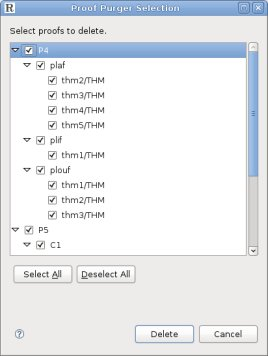
\includegraphics{img/reference/ref_10_proof_purger.png}
	\caption{Proof Purger Selection Window}
	\label{fig_ref_10_proof_purger}
\end{center}
\end{figure}

For the moment, nothing has been erased. The new window (see Figure \ref{fig_ref_10_proof_purger}) shows obsolete proofs and allows the user to choose among them and select the ones which should be deleted. One may wish to keep some of them knowing they might be useful in the future.

Once the selection has been decided, clicking the Delete button to actually delete the selected proofs from the proof files. Files that become empty will be deleted as well.

\subsubsection{Caution}

Proof purging should not be performed on models that are not in a stable state. For instance, it should not be applied to a model that has some errors or warnings issued by the type checker. This is because if there are errors and warnings, not all proof obligations are generated. Therefore, some proofs may have been considered wrongly as obsolete.
